% Quiz 08 --- Images and network surgery (the graph Laplacian). Printed, worked
% in class, 20 minutes, 10 points, one page. Answers are photographed and
% uploaded to the Google Form (go.skojaku.com/ans-quiz08), one photo per
% question.
%
% Question 1 treats a 5 x 5 pixel image (a 3 x 3 shaded square on a white
% background) as a 4-neighbor grid graph and asks students to compute Lx,
% showing that L takes local differences with neighbors and acts as an edge
% detector (giving 0 at the interior center pixel even though x_i = 1).
%
% Question 2 gives an 8-node double-diamond network with its Fiedler vector u
% printed beside the nodes (no degree-1 leaves, unique bridge D--E). Students
% choose (a) one edge to cut to disconnect the network and (b) one edge to add
% to maximize algebraic connectivity lambda_2, using sum_{(i,j) in E} (u_i - u_j)^2.
%
% The answers are in solutions.tex.
%
% Compile with: xelatex -interaction=nonstopmode quiz08.tex   (run twice)
\documentclass[a4paper, 11pt]{extarticle}
% Shared preamble for Quiz 08 (quiz08.tex and solutions.tex).
% Compile with: xelatex -interaction=nonstopmode <file>.tex   (run twice)
%
% Same house look as the pen-and-paper sheets in
% lecture-note/*/pen-and-paper/: Charter, A4, generous leading, room to draw.

\usepackage[top=0.7in, bottom=0.6in, left=0.8in, right=0.8in]{geometry}
\usepackage{amsmath}
\usepackage{amssymb}
\usepackage{array}
\usepackage{graphicx}
\usepackage[hidelinks]{hyperref}
\usepackage{tcolorbox}
\usepackage{enumitem}
\usepackage{etoolbox}
\usepackage{tikz}
\usepackage{fontspec}
\usetikzlibrary{calc,positioning,arrows.meta}
\definecolor{pltblue}{HTML}{1F77B4}
\definecolor{rulegrey}{HTML}{6A6D75}

% Body face. Charter, and the four ways to get it. XCharter *is* Charter and
% ships with a full TeX Live, so it is asked for first and by file: a CI runner
% answers yes to \IfFontExistsTF{Charter}, then cannot typeset it.
\IfFontExistsTF{XCharter-Roman.otf}{
  \setmainfont{XCharter}[
    Extension      = .otf,
    UprightFont    = *-Roman,
    BoldFont       = *-Bold,
    ItalicFont     = *-Italic,
    BoldItalicFont = *-BoldItalic]
}{
  \IfFontExistsTF{Charter}{\setmainfont{Charter}}{
    \IfFontExistsTF{Iowan Old Style}{\setmainfont{Iowan Old Style}}{
      \IfFontExistsTF{Georgia}{\setmainfont{Georgia}}{}}}}

\setlength{\parindent}{0pt}
\setlength{\parskip}{0.4em}
\setlength{\emergencystretch}{1.2em}
\raggedbottom
\pagestyle{empty}

% ---------------------------------------------------------------------------
% The submission link.
%
% Both the QR square and the printed address are the course's own short link,
% not the form's: paper outlives any one form. Caddy on the course droplet
% points go.skojaku.com/ans-quiz08 at the current Google Form
% (/etc/caddy/Caddyfile, block go.skojaku.com). Swapping the form is a line on
% the server, not a reprint.
%
% If the link ever changes, rebuild the square with
%
%   uvx --from segno segno --output=quiz08-form-qr.png --scale=20 --border=1 \
%       --error=m "<the url>"
% ---------------------------------------------------------------------------
\newcommand{\formlink}{https://go.skojaku.com/ans-quiz08}
\newcommand{\formshort}{\href{\formlink}{\texttt{go.skojaku.com/ans-quiz08}}}

% Quiz header. #1 = title, #2 = the line under it, #3 = term.
\newcommand{\quizhead}[3]{%
  {\footnotesize\textsc{Advanced Network Science} \hfill \textsc{#3}}\par
  \vspace{-0.2em}\rule{\textwidth}{1pt}\par
  \vspace{0.3em}
  {\LARGE\bfseries #1}\par
  \vspace{0.1em}
  {\small #2}\par
  \vspace{0.7em}
  {\small Name \underline{\hspace{6cm}} \hfill Date \underline{\hspace{3.2cm}}}\par
  \vspace{0.7em}}

% A question heading with its point value.
\newcommand{\question}[3]{%
  \vspace{0.5em}
  {\large\bfseries Question #1 \quad\normalsize\mdseries (#2 points)}\par
  \vspace{-0.3em}{\color{rulegrey}\rule{\textwidth}{0.6pt}}\par
  \vspace{0.1em}
  {\bfseries #3}\par
  \vspace{0.2em}}

% An empty box to draw or write in. #1 = height, #2 = caption under the rule.
\newcommand{\drawbox}[2]{%
  \begin{tcolorbox}[colback=white, colframe=rulegrey, boxrule=0.5pt,
                    sharp corners, height=#1, valign=top,
                    boxsep=2pt, left=4pt, right=4pt, top=3pt, bottom=3pt]
  {\footnotesize\color{rulegrey} #2}
  \end{tcolorbox}}

% Ruled writing lines, #1 of them.
\newcommand{\writelines}[1]{%
  \vspace{0.3em}
  \foreach \i in {1,...,#1}{%
    {\color{rulegrey}\rule{\textwidth}{0.4pt}}\par\vspace{1.5em}}}


% Title and points share one line, as in Quiz 5--7.
\renewcommand{\question}[3]{%
  \vspace{0.45em}
  {\large\bfseries Question #1 \quad #3\quad\normalsize\mdseries (#2 points)}\par
  \vspace{-0.4em}{\color{rulegrey}\rule{\textwidth}{0.6pt}}\par}

\tikzset{
  gnode/.style={circle, draw=pltblue, fill=pltblue!12, line width=0.9pt,
                minimum size=6.5mm, inner sep=0pt, font=\small\bfseries},
  gedge/.style={line width=0.9pt, draw=rulegrey},
  fval/.style={font=\footnotesize\ttfamily, text=black!80}
}

\begin{document}

\quizhead{Quiz 8 \; --- \; Images and network surgery}
        {20 minutes \quad$\cdot$\quad 10 points \quad$\cdot$\quad
         Closed notes}
        {Fall 2026}

\begin{tcolorbox}[colback=white, colframe=rulegrey, boxrule=0.5pt,
                  sharp corners, boxsep=1pt, top=4pt, bottom=4pt]
\begin{minipage}[c]{0.14\textwidth}
\begin{center}

\includegraphics[width=1.6cm]{quiz08-form-qr.png}
\end{center}
\end{minipage}
\hfill
\begin{minipage}[c]{0.83\textwidth}
{\small
Hand in two photos, one per question. Write each question's answer on
its own page, photograph each page, and upload it. \formshort.
}
\end{minipage}
\end{tcolorbox}

% ---------------------------------------------------------------------------
\question{1}{5}{What does the Laplacian do to an image?}

\begin{minipage}[c]{0.62\textwidth}
Treat the $5 \times 5$ pixel image on the right as a network of $N = 25$ nodes.
Two pixels share an edge if they touch horizontally or vertically (no diagonals).
Let $A$ be the adjacency matrix ($A_{ij} = 1$ if $i$ and $j$ share an edge, $0$
otherwise), $k_i = \sum_{j=1}^N A_{ij}$ be the degree of pixel $i$,
$D = \operatorname{diag}(k_1,\dots,k_N)$, and $L = D - A$ be the Laplacian.
Let $x = (x_1,\dots,x_N)^\top$ be the pixel values ($x_i = 1$ shaded, $x_i = 0$ white).
\end{minipage}
\hfill
\begin{minipage}[c]{0.34\textwidth}
\centering
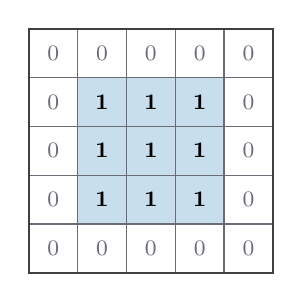
\begin{tikzpicture}[x=0.62cm, y=0.62cm]
  \foreach \r in {0,...,4} {
    \foreach \c in {0,...,4} {
      \ifnum\r>0 \ifnum\r<4 \ifnum\c>0 \ifnum\c<4
        \fill[pltblue!24] (\c, 4-\r) rectangle (\c+1, 5-\r);
        \node[font=\footnotesize\bfseries] at (\c+0.5, 4.5-\r) {1};
      \else
        \node[font=\footnotesize, text=rulegrey] at (\c+0.5, 4.5-\r) {0};
      \fi \else
        \node[font=\footnotesize, text=rulegrey] at (\c+0.5, 4.5-\r) {0};
      \fi \else
        \node[font=\footnotesize, text=rulegrey] at (\c+0.5, 4.5-\r) {0};
      \fi \else
        \node[font=\footnotesize, text=rulegrey] at (\c+0.5, 4.5-\r) {0};
      \fi
    }
  }
  \foreach \i in {1,...,4} {
    \draw[rulegrey, line width=0.5pt] (\i,0) -- (\i,5);
    \draw[rulegrey, line width=0.5pt] (0,\i) -- (5,\i);
  }
  \draw[black!75, line width=0.8pt] (0,0) rectangle (5,5);
\end{tikzpicture}
\end{minipage}

\medskip
(a) [1 pt] Show that $(Lx)_i = \sum_{j \in \mathcal{N}(i)} (x_i - x_j)$, where
$\mathcal{N}(i)$ is the set of neighbors of pixel $i$ and $(Lx)_i$ is entry $i$
of $Lx$.

\smallskip
(b) [2 pts] Compute $(Lx)_i$ for all $25$ pixels and write the result as a
$5 \times 5$ grid.

\smallskip
(c) [2 pts] What image feature does $Lx$ detect? Why is $(Lx)_i = 0$ at the
center pixel even though $x_i = 1$?

% ---------------------------------------------------------------------------
\vspace{0.3em}
\question{2}{5}{Network surgery.}

In the undirected network below ($N = 8$ nodes, edge set $E$), the number beside
each node $i$ is $u_i$, the $i$-th entry of the Fiedler vector
$u = (u_1,\dots,u_N)^\top$. Here $u$ is the unit eigenvector
($\sum_{i=1}^N u_i^2 = 1$) for the second smallest eigenvalue $\lambda_2 = 0.29$
of the Laplacian $L$, so
\[
  \lambda_2 \;=\; u^\top L u \;=\; \sum_{(i,j)\in E} (u_i - u_j)^2 ,
\]
where each undirected edge $(i,j) \in E$ is summed once.

\begin{center}
\vspace{-0.3em}
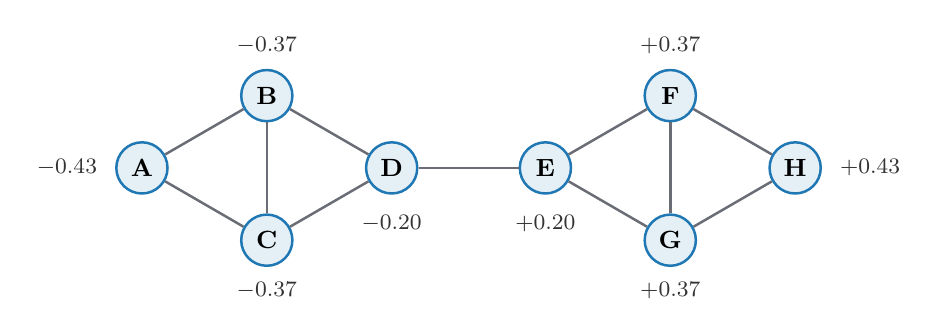
\begin{tikzpicture}[x=1.22cm, y=1.02cm]
  \node[gnode] (A) at (-3.4,  0.0) {A};
  \node[gnode] (B) at (-2.1,  0.9) {B};
  \node[gnode] (C) at (-2.1, -0.9) {C};
  \node[gnode] (D) at (-0.8,  0.0) {D};
  \node[gnode] (E) at ( 0.8,  0.0) {E};
  \node[gnode] (F) at ( 2.1,  0.9) {F};
  \node[gnode] (G) at ( 2.1, -0.9) {G};
  \node[gnode] (H) at ( 3.4,  0.0) {H};

  \foreach \a/\b in {A/B, A/C, B/C, B/D, C/D, D/E, E/F, E/G, F/G, F/H, G/H}
    \draw[gedge] (\a) -- (\b);

  \node[fval, left=3pt of A]  {$-0.43$};
  \node[fval, above=2pt of B] {$-0.37$};
  \node[fval, below=2pt of C] {$-0.37$};
  \node[fval, below=4pt of D] {$-0.20$};
  \node[fval, below=4pt of E] {$+0.20$};
  \node[fval, above=2pt of F] {$+0.37$};
  \node[fval, below=2pt of G] {$+0.37$};
  \node[fval, right=3pt of H] {$+0.43$};
\end{tikzpicture}
\vspace{-0.3em}
\end{center}

(a) [2 pts] Cut \textbf{one edge} to disconnect the network ($\lambda_2 = 0$).
Which edge is it, and how do the values $u_i$ identify it?

\smallskip
(b) [3 pts] Instead, add \textbf{one edge} to increase $\lambda_2$ as much as
possible. Which two nodes should you connect? Explain using
$\sum_{(i,j)\in E}(u_i - u_j)^2$.

\end{document}
